\xchapter{Revisão estruturada}{}

\subsection{Revisão estruturada} \label{revisao-estruturada}

\begin{figure}[h]
  \center
  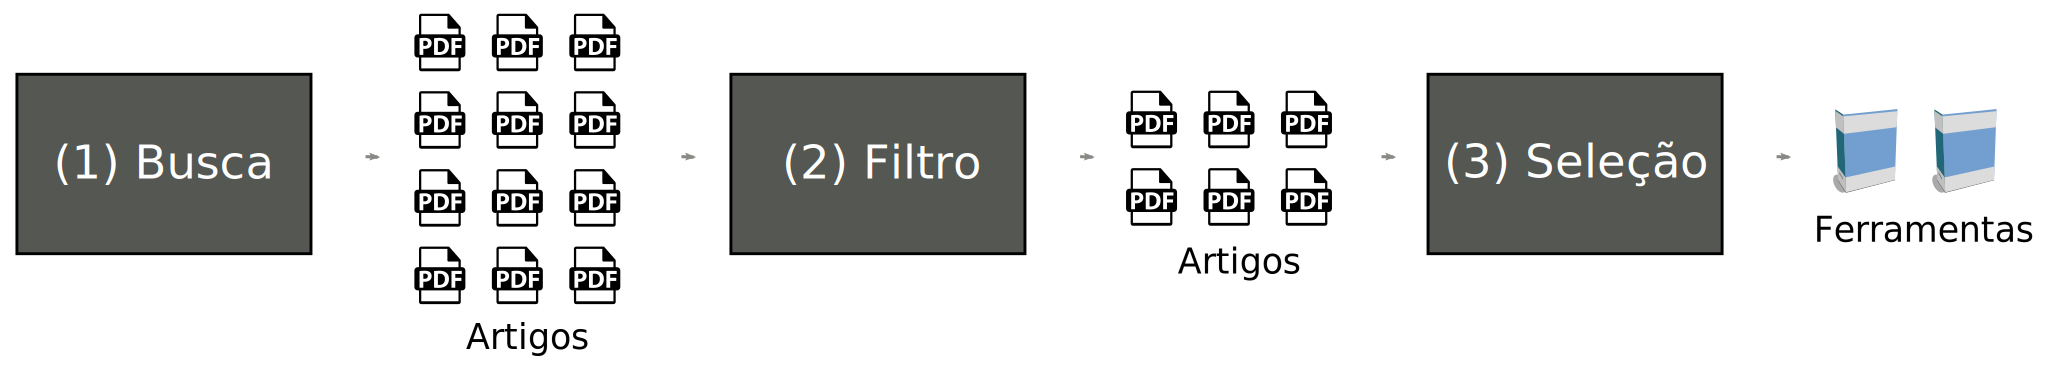
\includegraphics[scale=0.33]{imagens/revisao-estruturada.png}
  \caption{Representação gráfica da revisão estruturada}
  \label{figura-revisao-estruturada}
\end{figure}

A revisão estruturada é um processo disciplinado para seleção de artigos a
partir de critérios bem definidos, de forma que seja possível a reprodução do
estudo por parte de pesquisadores interessados.

A revisão está organizada em atividades de (1) busca de artigos (definição
das fontes de busca, definição de critérios de busca, definição de script de
busca, realização da busca nas fontes) e (2) seleção de artigos. 

No primeiro passo da revisão estruturada, as fontes de busca serão definidas,
considerando conferências que abordam o tema de interesse do estudo. 

A busca textual será realizada automaticamente, utilizando um
script\footnote{http://github.com/joenio/dissertacao-ufba-2016/blob/master/revisao-estruturada/filter}
escrito especialmente para este estudo. Esta busca seleciona os artigos que
contenham os seguintes termos:

\begin{verbatim}
  "tool" OU "framework"; E
  "download" OU "available"; E
  "http" OU "ftp"; E
  "static analysis" OU "parser".
\end{verbatim}

Uma cópia local de todos os artigos encontrados, em formato PDF, será feita.

No segundo passo, a seleção de artigos será feita com base nos artigos
encontrados pela busca no passo anterior.  Nesta seleção, pretende-se
identificar se cada artigo resulta, de fato, em publicação de ferramenta de
análise estática. Uma vez que se confirme que o artigo publica uma
ferramenta, este artigo será incluído para leitura. Ferramentas que sejam
mais abrangentes do que apenas análise estática mas que contenham esta função
em seu conjunto também serão selecionadas.

Uma vez identificados os artigos que publicaram ferramentas de análise
estática, procuramos no próprio artigo por referências de onde encontrar o
código-fonte da ferramenta. Neste contexto, algumas ações serão tomadas a
partir de algumas situações.

\begin{itemize}

  \item Se os autores afirmam que a ferramenta está disponível mas o artigo
    não contém referências de onde encontrar o código-fonte, então estes
    autores serão contactados, por email, solicitando informações de onde
    obter o código-fonte da ferramenta.

  \item Se o artigo indica onde obter o código-fonte da ferramenta, mas o acesso ao local
    indicado não está disponível, ou está disponível mas o software não se
    encontra lá, então os autores serão contactados, solicitando informações
    atualizadas de onde obter uma cópia do código-fonte da ferramenta.

  \item Artigos que indicam onde obter o código-fonte da ferramenta e a referência
    está correta. Será feito o download do código-fonte da última versão
    disponível.

\end{itemize}

Uma vez que os autores contactados por email respondam com informações sobre
local para obter o software, iremos adicionar a ferramenta ao conjunto de ferramentas
a serem analisadas.

Por fim, a ferramenta livre {\it
sloccount}\footnote{http://www.dwheeler.com/sloccount} será  utilizada para
identificar a linguagem de programação usada na implementação de cada
ferramenta selecionada.  A identificação da linguagem de programação é
necessária, pois apenas as ferramentas implementadas nas linguagens de
programação suportadas pela ferramenta Analizo serão consideradas.

\section{Coleta de dados} \label{coleta}

Serão realizadas duas etapas para identificar e mapear as ferramentas de
análise estática com código-fonte disponível: uma atividade para seleção de
ferramentas da academia, descrita na Seção \ref{ferramentas-da-academia}, e
outra atividade para seleção de ferramentas da indústria, descrita na Seção
\ref{ferramentas-da-industria}.

As ferramentas selecionadas para o estudo serão analisadas com Analizo para
extração dos valores de métricas de código-fonte.  Esta análise utilizará o
comando {\it metrics} do Analizo, que calcula métricas globais de projeto e
métricas por módulos. Este estudo levará em consideração a distribuição das
métricas por módulos.

\subsection{Ferramentas da academia} \label{ferramentas-da-academia}

A seleção de ferramentas da academia será relizada por meio de uma revisão
estruturada (seção~\ref{revisao-estruturada}). A fonte de busca para artigos
será a conferência SCAM - Source Code Analysis and Manipulation Working
Conference\footnote{http://www.ieee-scam.org} e mais uma dentre as seguintes
conferências:

\begin{itemize}
  \item ASE - Automated Software
    Engineering\footnote{http://ase-conferences.org}
  \item CSMR\footnote{A conferência CSMR tornou-se SANER - Software Analysis,
    Evolution, and Reengineering a partir da edição 2015.} - Conference on
    Software Maintenance and
    Reengineering\footnote{http://ansymore.uantwerpen.be/csmr-wcre}
  \item ICSME - International Conference on Software Maintenance and
    Evolution\footnote{http://www.icsme.org}
\end{itemize}

Todas estas conferências possuem trilhas para publicação de ferramentas e tem
como tema, áreas de estudo relacionadas à análise de programa e análise
estática, o que representa um grande potencial de encontrarmos ferramentas de
análise estática de código-fonte publicadas em suas mais de 20 edições. A
decisão de incluir apenas mais uma conferência além da conferência SCAM se
justifica pelo pouco tempo que temos para concluir este trabalho, de forma que
não seria viável incluir mais fontes.

Após download do código-fonte de cada ferramenta selecionada, em sua versão
mais recente, a ferramenta Analizo será utilizada para a coleta das métricas. 

\subsection{Ferramentas da indústria} \label{ferramentas-da-industria}

A seleção de ferramentas da indústria será feita de forma não estruturada a
partir de uma busca livre e manual no site do projeto SAMATE. As ferramentas
com código-fonte disponível, implementadas nas linguagens de programação
suportadas pelo Analizo serão selecionadas.

Após download do código-fonte de cada ferramenta selecionada, em sua versão
mais recente, a ferramenta Analizo será utilizada para a coleta das métricas. 

\section{Análise de dados} \label{analise}

Os dados coletados incluem métricas de código-fonte para cada módulo/classe de
cada ferramenta selecionada, tanto da indústria quanto da academia. As
métricas a serem analisadas e interpretadas são as métricas descritas na Seção
\ref{metricas-de-codigo}.

A linguagem R \cite{Ihaka1996}, uma linguagem de programação para cálculos
estatísticos e gráficos, será utilizada para manipulação de dados, criação de
tabelas e plotagem de gráficos. Todos os cálculos em linguagem R utilizados
neste trabalho estão disponíveis
em nosso repositório\footnote{https://github.com/joenio/dissertacao-ufba-2016/blob/master/qualificacao.R}.

\subsection{Distribuição dos valores das métricas}

Iremos calcular os percentis de cada métrica para cada ferramenta a partir dos
valores das métricas dos seus módulos, um percentil é a centésima parte dos
dados ordenados de forma crescente, iremos calcular os percentis 1, 5, 10, 25,
50, 75, 90, 95 e 99, e dentre eles iremos discutir os resultados em função dos
percentis 75, 90 e 95, assim como feito por \citeonline{Meirelles2013},
correspondendo a valores muito frequentes, frequentes e pouco frequentes,
respectivamente.

Esta discussão irá nos fornecer como resultado intervalos de referência para
métricas de código-fonte neste domínio de aplicação, estes intervalos serão
definidos a partir da interpretação manual dos percentis e serão analisados
usando modelos de regressão a fim de serem compreendidos e validados, uma
comparação com intervalos encontrados nos trabalhos relacionados (seção
\ref{trabalhos-relacionados}) também será realizada com objetivo de reforçar
estes valores.

\subsection{Cálculo de distância e modelo de aproximação} \label{distancia}

A partir da distribuição das métricas nos percentis 75, 90 e 95 e dos
intervalos de referência encontrados propomos uma abordagem para calcular o
quão distante cada ferramenta se encontra destes intervalos.  Esta abordagem
terá como base um fator de aproximação chamado {\it score} de similaridade,
este {\it score} será primeiramente calculado para os intervalos de referência
e servirão como base de comparação para o cálculo da distância de cada
ferramenta.

O {\it score} de similaridade será calculado a nível de projeto, ou seja,
teremos um único valor para cada ferramenta calculado a partir de suas várias
métricas. Para isto, iremos abstrair o significado individual de cada métrica,
o que pode não ser muito efetivo já que diferentes métricas possuem diferentes
grandezas. Para resolver este problema será feita uma normalização dos valores
das várias métricas a fim de deixá-las num mesmo intervalo, com uma certa
equivalência, seguindo uma ideia semelhante ao que é feito com a distância
euclidiana, onde todas as variáveis tem suas distâncias unificadas em um único
valor.

Os valores do {\it score} calculados a partir dos intervalos de referência
serão centralizados em 0, indicando o centro de comparação para o cálculo da
distância com cada ferramenta, desta forma, ferramentas com {\it score} acima
de 0 indicam valores piores em relação aos intervalos de referência, e
ferramentas com {\it score} abaixo de 0 indicam valores melhores do que os
intervalos de referência.

%(+ metodologia)
% apresentar parte da metodologia aqui
% e documentar a revisao estruturada em detalhes
% mover conteudo da antiga metodolgia pra cá, o que for relacionado a revisao

Foi feito download de todos os artigos em formato PDF de todas as edições das
conferências SCAM - Source Code Analysis and Manipulation Working
Conference\footnote{http://www.ieee-scam.org} e ASE - Automated Software
Engineering Conference\footnote{http://ase-conferences.org}.
Os artigos foram organizados por edição em pastas separadas para posterior
seleção automatizada via script\footnote{http://github.com/joenio/dissertacao-ufba-2016/blob/master/revisao-estruturada/filter} desenvolvido com objetivo de filtrar os
artigos por palavras-chaves, os resultados desta primeira seleção são apresentados
na seção \ref{artigos-selecionados-filter}.

Seguem os artigos copiados localmente para posterior filtro e seleção.

Numa primeira seleção de forma automatizada através do script "filter" foram
selecionados 436 artigos. Organizados à seguir separados por conferência e
edição, os artigos selecionados nesta primeira etapa estão marcados na lista
abaixo com um {\color{blue} \checkmark}. Os artigos selecionados nas duas
etapas serão marcados com dois {\color{blue} \checkmark \checkmark}.

Artigos que citam que desenvolveram alguma ferramenta, protótipo ou prova de
conceito mas não dão nenhum detalhes sobre a ferramenta, como nome ao menos,
não serão incluídos na caracterização das ferramentas e será listado aqui como
{\color{blue} \checkmark}{\color{red} \texttimes}. Ou seja, estarão excluídos
da segunda fase de seleção manual realizada através de uma leitura superficial
do artigo em busca de informações sobre publicação de ferramenta.

%# Papers tools da conferencia estao no IEEE Xplore?
%
%(enviei em 16/nov email para os chairs da trilha ferramentas do SCAM 2014
%perguntando onde encontro os papers da trilha ferramentas)
%
%17/11 - Foutse Khomh respondeu informando que no IEEEXplore tem tudo,
%incluindo os tools papers.
%
%uma leitura superficial
%para encontrar referencia e link sobre ferramenta desenvolvida
%resultou nos seguintes papers com ferramenta disponível livremente:
%
%SCAM 2010/05601817.pdf Wrangler (OK) - mas erlang nao pode ser analisado
%
%9 novas ferramentas, verificar qual linguagem é utilizada em cada uma delas:
%
%* Wrangler        | erlang
%
%Podemos analizar todas exceto Wrangler em erlang, então são 9 ferramentas.
%Somando a ferramenta SourceMeter encontrada no levantamento anterior dos anos
%2001, 2002, 2013, 2014. Temos total de 9 ferramentas da academia para anlisar.

\section{SCAM - Source Code Analysis and Manipulation Working Conference}

Todos os artigos em formato PDF foram obtidos de forma manual através da área
da conferência SCAM no IEEE
Xplore\footnote{http://ieeexplore.ieee.org/xpl/conhome.jsp?punumber=1000715}.

\subsection{SCAM 2001}

{\small \em http://ieeexplore.ieee.org/xpl/mostRecentIssue.jsp?punumber=7667}


\subsection{SCAM 2002}

{\small \em http://ieeexplore.ieee.org/xpl/mostRecentIssue.jsp?punumber=6494367}


\subsection{SCAM 2003}

{\small \em http://ieeexplore.ieee.org/xpl/mostRecentIssue.jsp?punumber=8773}

\subsection{SCAM 2004}

{\small \em http://ieeexplore.ieee.org/xpl/mostRecentIssue.jsp?punumber=9523}

\subsection{SCAM 2005}

{\small \em http://ieeexplore.ieee.org/xpl/mostRecentIssue.jsp?punumber=10344}

\subsection{SCAM 2006}

{\small \em http://ieeexplore.ieee.org/xpl/mostRecentIssue.jsp?punumber=4026839}


\subsection{SCAM 2007}

{\small \em http://ieeexplore.ieee.org/xpl/mostRecentIssue.jsp?punumber=4362882}

\subsection{SCAM 2008}

{\small \em http://ieeexplore.ieee.org/xpl/mostRecentIssue.jsp?punumber=4637522}

\subsection{SCAM 2009}

{\small \em http://ieeexplore.ieee.org/xpl/mostRecentIssue.jsp?punumber=5279860}

\subsection{SCAM 2010}

{\small \em http://ieeexplore.ieee.org/xpl/mostRecentIssue.jsp?punumber=5600365}

\subsection{SCAM 2011}

{\small \em http://ieeexplore.ieee.org/xpl/mostRecentIssue.jsp?punumber=6063701}

\subsection{SCAM 2012}

{\small \em http://ieeexplore.ieee.org/xpl/mostRecentIssue.jsp?punumber=6389882}

\subsection{SCAM 2013}

{\small \em http://ieeexplore.ieee.org/xpl/mostRecentIssue.jsp?punumber=6636284}

\subsection{SCAM 2014}

{\small \em http://ieeexplore.ieee.org/xpl/mostRecentIssue.jsp?punumber=6970367}

\subsection{SCAM 2015}

{\small \em http://ieeexplore.ieee.org/xpl/mostRecentIssue.jsp?punumber=7321933}

\section{ASE - Automated Software Conference}

Até o ano de 1996 a conferencia ASE se chamava KBSE - Knowledge-Based Software
Engineering
Conference\footnote{http://ieeexplore.ieee.org/xpl/conhome.jsp?punumber=1000410}
e a partir de 1997 passou a se chamar ASE - Automated Software
Conference\footnote{http://ieeexplore.ieee.org/xpl/conhome.jsp?punumber=1000064}.
A maioria das edições estão disponíveis no IEEE Xplore, mas algumas outras
estão no ACM Digital Library, em cada sub-seção será indicado onde os arquivos
PDF foram obtidos.

\subsection{ASE/KBSE 1991}

{\small \em http://ieeexplore.ieee.org/xpl/mostRecentIssue.jsp?punumber=5069}

\subsection{ASE/KBSE 1992}

{\small \em http://ieeexplore.ieee.org/xpl/mostRecentIssue.jsp?punumber=421}

\subsection{ASE/KBSE 1993}

{\small \em http://ieeexplore.ieee.org/xpl/mostRecentIssue.jsp?punumber=921}

\subsection{ASE/KBSE 1994}

{\small \em http://ieeexplore.ieee.org/xpl/mostRecentIssue.jsp?punumber=995}

\subsection{ASE/KBSE 1995}

{\small \em http://ieeexplore.ieee.org/xpl/mostRecentIssue.jsp?punumber=3518}

\subsection{ASE/KBSE 1996}

{\small \em http://ieeexplore.ieee.org/xpl/mostRecentIssue.jsp?punumber=4065}

\subsection{ASE 1997}

{\small \em http://ieeexplore.ieee.org/xpl/mostRecentIssue.jsp?punumber=5003}

\subsection{ASE 1998}

{\small \em http://ieeexplore.ieee.org/xpl/mostRecentIssue.jsp?punumber=5935}

\subsection{ASE 1999}

{\small \em http://ieeexplore.ieee.org/xpl/mostRecentIssue.jsp?punumber=6516}

\subsection{ASE 2000}

{\small \em http://ieeexplore.ieee.org/xpl/mostRecentIssue.jsp?punumber=7013}

\subsection{ASE 2001}

{\small \em http://ieeexplore.ieee.org/xpl/mostRecentIssue.jsp?punumber=7763}

\subsection{ASE 2002}

{\small \em http://ieeexplore.ieee.org/xpl/mostRecentIssue.jsp?punumber=8183}

\subsection{ASE 2003}

{\small \em http://ieeexplore.ieee.org/xpl/conhome.jsp?punumber=1000064}

\subsection{ASE 2004}

{\small \em http://ieeexplore.ieee.org/xpl/mostRecentIssue.jsp?punumber=9305}

\subsection{ASE 2005}

{\small \em http://dl.acm.org/citation.cfm?id=1101908}

\subsection{ASE 2006}

{\small \em http://ieeexplore.ieee.org/xpl/mostRecentIssue.jsp?punumber=4019543}

\subsection{ASE 2007}

{\small \em http://dl.acm.org/citation.cfm?id=1321631}

\subsection{ASE 2008}

{\small \em http://ieeexplore.ieee.org/xpl/mostRecentIssue.jsp?punumber=4639292}

\subsection{ASE 2009}

{\small \em http://ieeexplore.ieee.org/xpl/mostRecentIssue.jsp?punumber=5431684}

\subsection{ASE 2010}

{\small \em http://dl.acm.org/citation.cfm?id=1858996}

\subsection{ASE 2011}

{\small \em http://ieeexplore.ieee.org/xpl/mostRecentIssue.jsp?punumber=6093623}

\subsection{ASE 2012}

{\small \em http://ieeexplore.ieee.org/xpl/mostRecentIssue.jsp?punumber=6494367}

\subsection{ASE 2013}

{\small \em http://ieeexplore.ieee.org/xpl/mostRecentIssue.jsp?punumber=6684409}

\subsection{ASE 2014}

{\small \em http://dl.acm.org/citation.cfm?id=2642937}

\subsection{ASE 2015}

{\small \em http://ieeexplore.ieee.org/xpl/mostRecentIssue.jsp?punumber=7371449}

